\section{Classificação de recursos no \emph{middleware uOS}}
\label{sec:classificacaoNoUos}

O \emph{uOS} é um \emph{middleware} cujo propósito é fornecer uma infra-estrutura de software utilizando conceitos de computação ubíqua com foco na adaptabilidade de serviços. Seguindo a arquitetura \emph{DSOA}, o \emph{uOS} é responsável por dar suporte para o desenvolvimento de \emph{drivers} e aplicações. Além disso, o \emph{uOS} utiliza o conjunto de protocolos \emph{uP} para realizar sua comunicação.

\begin{figure}[ht]
	\center
	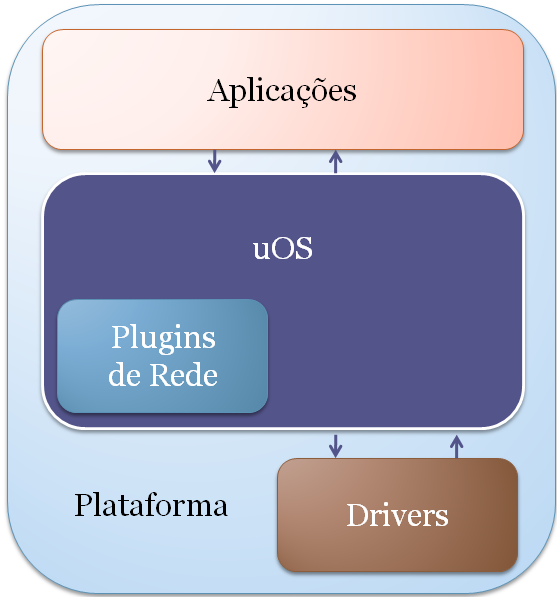
\includegraphics[scale=0.4]{imagens/ecossistemaUbiquitos}
	\caption{Ecossistema do \emph{uOS}.}
	\label{fig:ecossistemaUbiquitos}
\end{figure}

A Figura~\ref{fig:ecossistemaUbiquitos} mostra o ecossistema do \emph{middleware}, em que os \emph{plugins} de rede, abstrações para a rede de comunicação, se destacam como um componente dentro do \emph{uOS}. O \emph{middleware}, por sua vez, utiliza os \emph{plugins} para interfacear a comunicação entre aplicações, por meio de \emph{drivers}. No sistema destacam-se três camadas: Rede, Conectividade e Adaptabilidade. A camada de Adaptabilidade é responsável pela coordenação de interaçòes feitas por meio do \emph{middleware}. A Figura~\ref{fig:diagramaDeBlocos} mostra a arquitetura interna da camada de adaptabilidade do \emph{uOS}.

\begin{figure}[ht]
	\center
	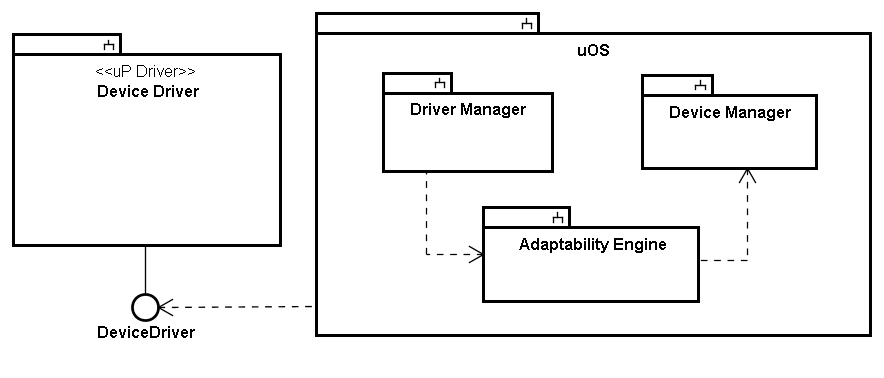
\includegraphics[scale=0.6]{imagens/diagramaDeBlocos}
	\caption{Arquitetura interna da camada de adaptabilidade do \emph{uOS}.}
	\label{fig:diagramaDeBlocos}
\end{figure}

No \emph{Driver Manager} foi adicionada uma estrutura em forma de floresta, em que a raiz de cada árvore representa um recurso novo que não é equivalente a nenhum outro. Essa estrutura é inicializada juntamente com o \emph{Driver Manager} com cada tipo básico, conforme definido na Seção~\ref{sec:tiposBasicos} compondo uma nova raiz da estrutura de árvores. Este componente é responsável por manter as relações de equivalência dos recursos, mantendo a consistência de serviços e interfaces e impedindo que ocorra uma referência circular entre recursos equivalentes. Quando um novo recurso é registrado no \emph{middleware}, este \emph{manager} realiza validações em seu \emph{driver} segundo as relações de quivalência e em seguida o \emph{driver} é adicionado na árvore de equivalência correta. 

Além de manter essa estrutura, o \emph{Driver Manager} é responsável por popular a ontologia do \emph{uOS}. O novo \emph{driver} é adicionado à ontologia utilizando a \emph{uOS-Context API}, um conjunto de interfaces que permite a manipulação estrutural e semântica da Ontologia de Contexto do \emph{uOS}~\cite{ozakisbcup2011}. Na Figura~\ref{fig:ontologiaUOS} observa-se uma ontologia que contém as classes dos recursos \emph{Pointer} e \emph{Keyboard}.

\begin{figure}[ht]
	\center
	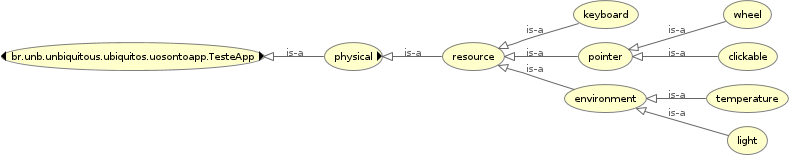
\includegraphics[scale=0.7]{imagens/ontologia}
	\caption{Exemplo de recursos da Ontologia do \emph{uOS}.}
	\label{fig:ontologiaUOS}
\end{figure}

Na camada de adaptabilidade, Figura~\ref{fig:diagramaDeBlocos}, o \emph{Device Manager} é responsável pela gerenciamento de dispositivos presentes no ambiente, ou seja, este componente é notificado por um radar sobre a entrada ou saída de dispositivos e o \emph{Driver Manager}, responsável por determinar o \emph{driver} de recurso irá tratar uma chamada recebida pela \emph{Message Engine}, responsável por traduzir dados da camada de rede em objetos compreendidos pelas demais camadas.

O processo de \emph{handshake}, no qual ocorre a descoberta de novos recursos do ambiente, foi alterado visando tratar os casos em que equivalências desconhecidas são encontradas. Visando um melhor desempenho, foi adicionada uma nova fase ao processo para se tratar estes casos. Quando um novo recurso a ser registrado é equivalente a pelo menos um recurso desconhecido, o \emph{Driver Manager} não irá registrá-lo em sua árvore de equivalência enquanto não conhecê-lo. Neste caso, o módulo \emph{Device Manager} é responsável por descobrir esse(s) recurso(s). Após conhecer a interface dos recursos, este módulo irá então registrar cada recurso desconhecido para então registrar o novo recurso na árvore de equivalência. Para que o \emph{Device Manager} possa descobrir a interface de um determinado recurso desconhecido ele deve procurar o dispositivo que possui este recurso. Para prover esta informação, foi criado o protocolo complementar \emph{``tellEquivalentDrivers''} dentro do \emph{Device Driver}. Este é responsável por informar a interface de todos os recursos necessários para que o registro no \emph{uOS} possa ocorrer.